\chapter{Avancement général}

En raison de l'abandon du projet par Thibaud LE DOLEDEC et Clément AILLOUD partis en stage, le projet ne pourra être mené à terme. Pour aborder la dernière ligne droite avant l'évaluation finale, un choix a donc été fait des taches sur lesquelles travailler en priorité, au détriment d'autres qui demeureront inachevées.

\vspace{1cm}

Ci-dessous un diagramme représentant l’avancement des différentes taches du projet. Le gris indique qu’une tache est terminée ou à un niveau d’avancement satisfaisant et garantissant une maturité proche. Le orange indique les taches sur lesquelles nous travaillerons en priorité avant la fin du projet. Les flèches représentent des liens de dépendance entre les taches.

\begin{figure}[H]
    \centering
	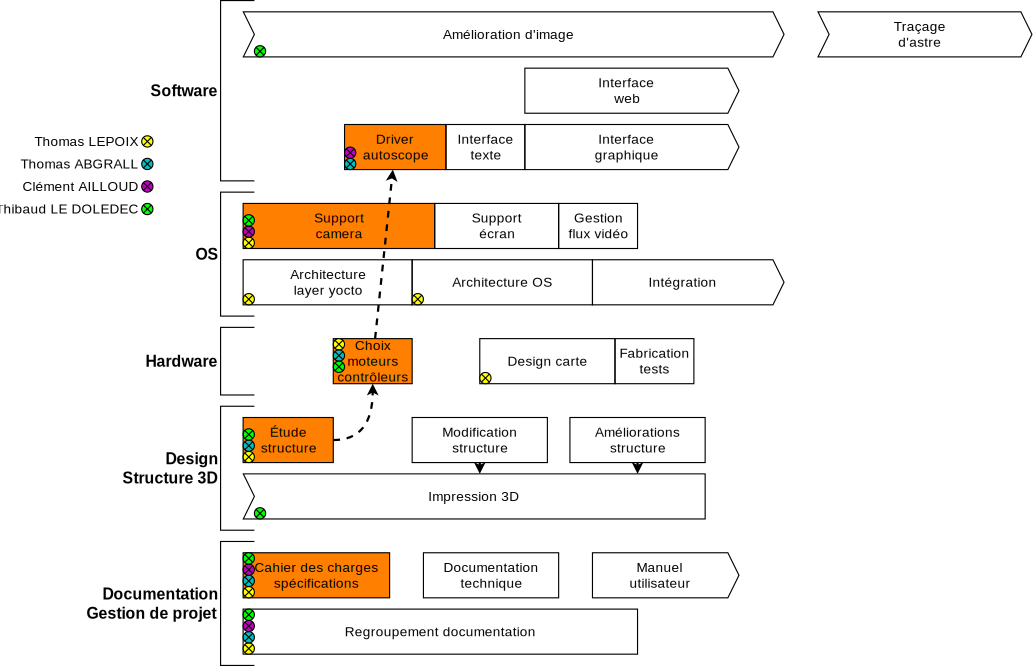
\includegraphics[width=1\linewidth]{\figures/sch_gantt.pdf}
    \decoRule
    \caption[
    Diagramme de l'organisation temporelle du travail sur le projet]{
    Diagramme de l'organisation temporelle du travail sur le projet}
    \label{fig:Diagramme de l'organisation temporelle du travail sur le projet}
    \end{figure}

\section{Prévisions pour le dernier sprint}

Malgré son aspect visuel intéressant pour promouvoir le projet ainsi que de sont aspect central (il s'agit tout de même d'un télescope), le travail sur la structure du télescope sera écarté des taches prioritaires. Cela pour deux raisons~:
\begin{itemize}[label=$\bullet$]
	\item Il s'agit d'une partie du projet demandant beaucoup de temps et d'implications par rapport à ce dont nous disposons. Nous n'aurions sans doute pas le temps de terminer cela avant l'évaluation.
	\item N'ayant ni des connaissances particulières en optique, ni la maîtrise d'un logiciel de modélisation 3D, nous ne sommes pas plus qualifiés qu'une personne aléatoire voulant contribuer au projet. Nous pensons donc qu'il vaut mieux nous concentrer sur des taches faisant partie de notre domaine de qualification, que nous serions capable de réaliser plus facilement ou mieux qu'une personne aléatoire. L'élaboration des drivers correspond typiquement à ce cas.
	\end{itemize}

\vspace{1cm}

Le travail sur les drivers, quant à lui devra être avancé autant que faire se peut. En effet le logiciel principal du télescope dépend lourdement des interfaces avec les drivers et ne peut être commencé tant que les drivers ne sont pas fonctionnels.

De plus, ce logiciel étant la clef de voûte du projet, la finalisation de certaines taches comme certains éléments du plugin Stellarium ou la gestion du flux vidéo au sein de l'OS doit être réalisée conjointement à l'écriture de ce logiciel.

L'absence des ces drivers commence donc à bloquer l'évolution d'autres taches.

\vspace{1cm}

Enfin un travail de documentation devra être fait pour qu'il soit possible à une personne future (nous-mêmes ou qui que ce soit) de travailler sur ce projet ou de réutiliser notre travail.




